\documentclass{article}
\usepackage{graphicx}
\usepackage{hyperref}

\title{Travel To The Moon}
\author{}
\date{}

\renewcommand{\labelenumi}{\arabic{enumi}.}
\renewcommand{\labelenumii}{\arabic{enumi}.\arabic{enumii}.}
\renewcommand{\labelenumiii}{\arabic{enumi}.\arabic{enumii}.\arabic{enumiii}.}
\renewcommand{\labelenumiv}{\arabic{enumi}.\arabic{enumii}.\arabic{enumiii}.\arabic{enumiv}.}
\begin{document}

\maketitle

\section{Specifiche del progetto}

I dati di interesse per il sistema sono le crociere offerte dall'agenzia con le relative prenotazioni e le destinazioni in catalogo.
\\
Il sistema deve essere in grado di rappresentare le crociere offerte dall'agenzia, con codice, date di inizio e fine, e la nave utilizzata. Delle navi, che hanno un nome (ad es. LoveBoat), interessa il grado di comfort, espresso in un numero di stelle che può variare da 3 a 5, e il numero massimo di passeggeri che possono ospitare.
\\
Ciascuna crociera consta di un itinerario caratterizzato da un nome (ad es. Panorami d'Oriente) il quale prevede una sequenza ordinata di destinazioni. Di queste interessa il nome e il continente in cui si trovano. Gli itinerari fissano, oltre che l'ordine delle destinazioni da visitare, anche la relativa data ed ora di arrivo e di partenza. Dato che, in generale, un itinerario può essere previsto da più di una crociera, le date di arrivo e partenza relative ad una destinazione vengono espresse come differenze rispetto la data di inizio della crociera stessa (ad es., l'itinerario Panorami d'Oriente prevede di raggiungere la destinazione x alle 16:00 del quinto giorno di crociera, e di ripartire alle 12:00 del giorno successivo, il sesto).
\\
Inoltre, le destinazioni sono caratterizzate da un insieme di posti da vedere durante eventuali escursioni organizzate. Questi ultimi sono caratterizzati dal nome, dalla descrizione, e dalla fascia oraria consigliata per le visite. Il sistema deve permettere di risalire ai posti da vedere in ogni singola destinazione.
\\
L'agenzia classifica le crociere in crociere di luna di miele e crociere per famiglia (di queste ultime interessa conoscere se sono adatte o meno ai bambini), e le destinazioni in romantiche e divertenti. Si noti che possono esistere destinazioni che sono sia romantiche che divertenti. Per venire incontro alle nuove tendenze delle giovani coppie, le crociere di luna di miele vengono ulteriormente classificate in tradizionali e alternative: sono definite tradizionali quelle che prevedono un numero di destinazioni romantiche maggiore o uguale al numero di destinazioni divertenti, alternative le altre.
\\
Infine, il sistema deve anche permettere di gestire le prenotazioni di crociere effettuate dai clienti. In particolare, dei clienti interessa nome, cognome, età ed indirizzo, mentre delle prenotazioni interessa l'istante di prenotazione, la crociera ed il numero di posti prenotati.
\\

Le funzionalità richieste al sistema sono le seguenti:

\begin{enumerate}
    \item Dato un cliente che desidera prenotare un certo numero di posti per una crociera c, il personale dell'Ufficio Prenotazioni deve poter effettuare la relativa prenotazione. La richiesta di prenotazione deve essere rifiutata nel caso il numero di posti disponibili, all'istante corrente, per la crociera c non sia sufficiente.
    \item L'Ufficio Marketing deve poter calcolare l'età media dei clienti che hanno prenotato, in un dato periodo, almeno una crociera che prevede una destinazione esotica (ovvero che si trova in un continente diverso dall'Europa).
    \item L'Ufficio Marketing deve poter calcolare la percentuale delle destinazioni da considerarsi gettonate in un periodo dato. Una destinazione va considerata gettonata in un certo periodo se è stata raggiunta, in quel periodo, da almeno dieci crociere di luna di miele, oppure da almeno quindici crociere per famiglie.
\end{enumerate}

\newpage
\section{Raffinamento dei requisiti}

In questa sezione verranno descritte le fasi di raffinamento dei requisiti.

\begin{enumerate}
    \item Requisiti sulle \hyperref[sec:Crociera]{crociere}\label{sec:RequisitiCrociera}
    \begin{enumerate}
        \item codice: \hyperref[sec:StringaS]{StringaS}\label{sec:RequisitiCrocieraCodice}
        \item data di inizio: Data\label{sec:RequisitiCrocieraDataInizio}
        \item data di fine: Data\label{sec:RequisitiCrocieraDataFine}
        \item nave utilizzata (\hyperref[sec:RequisitiNave]{v.req.2})\label{sec:RequisitiCrocieraNave}
        \item itinerario (\hyperref[sec:RequisitiItinerario]{v.req.4})\label{sec:RequisitiCrocieraItinerario}
        \item Le prenotazioni (v.req.7)\label{sec:RequisitiCrocieraPrenotazioni}
        \item il tipo, uno tra:\label{sec:RequisitiCrocieraTipo}
        \begin{enumerate}
            \item crociera di luna di miele, di cui interessa:\label{sec:RequisitiCrocieraTipoLunaDiMiele}
            \begin{enumerate}
                \item tradizionale\label{sec:RequisitiCrocieraTipoLunaDiMieleTradizionale}
                \item alternativa\label{sec:RequisitiCrocieraTipoLunaDiMieleAlternativa}
            \end{enumerate}
            \item crociera per famiglie\label{sec:RequisitiCrocieraTipoPerFamiglie}
            \begin{enumerate}
                \item adatta ai bambini: booleano\label{sec:RequisitiCrocieraTipoPerFamiglieAdattaAiBambini}
            \end{enumerate}
        \end{enumerate}
    \end{enumerate}
    \item Requisiti sulle \hyperref[sec:Nave]{navi}\label{sec:RequisitiNave}
    \begin{enumerate}
        \item nome: \hyperref[sec:StringaS]{StringaS}\label{sec:RequisitiNaveNome}
        \item grado di comfort (da 3 a 5 stelle): \hyperref[sec:ValutazioneNave]{ValutazioneNave}\label{sec:RequisitiNaveGradoDiComfort}
        \item numero massimo di passeggeri: InteroGZ\label{sec:RequisitiNaveNumeroMassimoDiPasseggeri}
        \item le crociere che fanno uso della nave (\hyperref[sec:RequisitiCrociera]{\hyperref[sec:RequisitiCrociera]{v.req.1}})\label{sec:RequisitiNaveCrociere}
    \end{enumerate}
    \item Requisiti sulle \hyperref[sec:Destinazione]{destinazioni}\label{sec:RequisitiDestinazione}
    \begin{enumerate}
        \item nome: \hyperref[sec:StringaS]{StringaS}\label{sec:RequisitiDestinazioneNome}
        \item la città in cui si trova (\hyperref[sec:RequisitiCittà]{v.req.8})\label{sec:RequisitiDestinazioneCittà}
        \item posti da vedere (\hyperref[sec:RequisitiPostoDaVedere]{v.req.5})\label{sec:RequisitiDestinazionePostiDaVedere}
        \item i porti dai quali può essere raggiunta (\hyperref[sec:RequisitiPorto]{v.req.11})\label{sec:RequisitiDestinazionePorti}
        \item Il tipo, uno o entrambe tra:\label{sec:RequisitiDestinazioneTipo}
        \begin{enumerate}
            \item romantica\label{sec:RequisitiDestinazioneTipoRomantica}
            \item divertente\label{sec:RequisitiDestinazioneTipoDivertente}
        \end{enumerate}
    \end{enumerate}
    \item Requisiti sugli \hyperref[sec:Itinerario]{itinerari}\label{sec:RequisitiItinerario}
    \begin{enumerate}
        \item nome: \hyperref[sec:StringaS]{StringaS}\label{sec:RequisitiItinerarioNome}
        \item le tappe (\hyperref[sec:RequisitiTappa]{v.req.13})\label{sec:RequisitiItinerarioTappe}
        \item destinazione di partenza (\hyperref[sec:RequisitiDestinazione]{v.req.3})\label{sec:RequisitiItinerarioDestinazioneDiPartenza}
        \begin{enumerate}
            \item ora di partenza: Ora\label{sec:RequisitiItinerarioDestinazioneDiPartenzaOra}
        \end{enumerate}
        \item destinazione di arrivo (\hyperref[sec:RequisitiDestinazione]{v.req.3})\label{sec:RequisitiItinerarioDestinazioneDiArrivo}
        \begin{enumerate}
            \item ora di arrivo: Ora\label{sec:RequisitiItinerarioDestinazioneDiArrivoOra}
            \item giorno di arrivo (rappresentato come differenza rispetto la data di inizio della crociera): InteroGEZ\label{sec:RequisitiItinerarioPortoDiArrivoGiorno}
        \end{enumerate}
    \end{enumerate}
    \item Requisiti sui \hyperref[sec:PostoDaVedere]{posti da vedere}\label{sec:RequisitiPostoDaVedere}
    \begin{enumerate}
        \item nome: \hyperref[sec:StringaS]{StringaS}\label{sec:RequisitiPostoDaVedereNome}
        \item descrizione: \hyperref[sec:StringaL]{StringaL}\label{sec:RequisitiPostoDaVedereDescrizione}
        \item fascia oraria consigliata (\hyperref[sec:RequisitiOrarioPostoDaVedere]{v.req.11})\label{sec:RequisitiPostoDaVedereFasciaOrariaConsigliata}
        \item la città in cui si trovano (\hyperref[sec:RequisitiCittà]{v.req.8})\label{sec:RequisitiPostoDaVedereCittà}
    \end{enumerate}
    \item Requisiti sugli utenti\label{sec:RequisitiUtente}
    \begin{enumerate}
        \item nome: \hyperref[sec:StringaS]{StringaS}\label{sec:RequisitiUtenteNome}
        \item cognome: \hyperref[sec:StringaS]{StringaS}\label{sec:RequisitiUtenteCognome}
        \item indirizzo: \hyperref[sec:StringaM]{StringaM}\label{sec:RequisitiUtenteIndirizzo}
        \item data di nascita: Data\label{sec:RequisitiUtenteDataDiNascita}
        \item città di residenza (\hyperref[sec:RequisitiCittà]{v.req.8})\label{sec:RequisitiUtenteCittàDiResidenza}
    \end{enumerate}
    \item Requisiti sulle \hyperref[sec:Prenotazione]{prenotazioni}\label{sec:RequisitiPrenotazione}
    \begin{enumerate}
        \item istante di prenotazione: Dataora\label{sec:RequisitiPrenotazioneIstanteDiPrenotazione}
        \item crociera prenotata (\hyperref[sec:RequisitiCrociera]{v.req.1})\label{sec:RequisitiPrenotazioneCrocieraPrenotata}
        \item numero di posti prenotati: \hyperref[sec:InteroGZ]{InteroGZ}\label{sec:RequisitiPrenotazioneNumeroDiPostiPrenotati}
        \item l'utente che ha effettuato la prenotazione (\hyperref[sec:RequisitiUtente]{v.req.6})\label{sec:RequisitiPrenotazioneUtente}
    \end{enumerate}
    \item Requisiti sulle \hyperref[sec:Città]{città}\label{sec:RequisitiCittà}
    \begin{enumerate}
        \item nome: \hyperref[sec:StringaS]{StringaS}\label{sec:RequisitiCittàNome}
        \item la nazione in cui si trova (\hyperref[sec:RequisitiNazione]{v.req.9})\label{sec:RequisitiCittàNazione}
    \end{enumerate}
    \item Requisiti sulle \hyperref[sec:Nazione]{nazioni}\label{sec:RequisitiNazione}
    \begin{enumerate}
        \item nome: \hyperref[sec:StringaS]{StringaS}\label{sec:RequisitiNazioneNome}
        \item il continente in cui si trova (\hyperref[sec:RequisitiContinente]{v.req.10})\label{sec:RequisitiNazioneContinente}
    \end{enumerate}
    \item Requisiti sui \hyperref[sec:Continente]{continenti}\label{sec:RequisitiContinente}
    \begin{enumerate}
        \item nome: \hyperref[sec:StringaS]{StringaS}\label{sec:RequisitiContinenteNome}
    \end{enumerate}
    \item Requisiti sui \hyperref[sec:Porto]{porti}\label{sec:RequisitiPorto}
    \begin{enumerate}
        \item nome: \hyperref[sec:StringaS]{StringaS}\label{sec:RequisitiPortoNome}
        \item la destinazione (0 o 1) (\hyperref[sec:RequisitiDestinazione]{v.req.3})\label{sec:RequisitiPortoDestinazione}
        \item la città in cui si trova (\hyperref[sec:RequisitiCittà]{v.req.8})\label{sec:RequisitiPortoCittà}
    \end{enumerate}
    \item Requisiti sugli \hyperref[sec:OrarioPostoDaVedere]{orari dei posti da vedere}\label{sec:RequisitiOrarioPostoDaVedere}
    \begin{enumerate}
        \item giorno: \hyperref[sec:Giorno]{Giorno}\label{sec:RequisitiOrarioPostoDaVedereGiorno}
        \item ora di inizio: \hyperref[sec:Ora]{Ora}\label{sec:RequisitiOrarioPostoDaVedereOraDiInizio}
        \item ora di fine: \hyperref[sec:Ora]{Ora}\label{sec:RequisitiOrarioPostoDaVedereOraDiFine}
    \end{enumerate}
    \item Requisiti delle \hyperref[sec:Tappa]{tappe degli itinerari}\label{sec:RequisitiTappa}
    \begin{enumerate}
        \item l'itinerario (\hyperref[sec:RequisitiItinerario]{v.req.4})\label{sec:RequisitiTappaItinerario}
        \item la destinazione (\hyperref[sec:RequisitiDestinazione]{v.req.3})\label{sec:RequisitiTappaDestinazione}
        \item il giorno di arrivo (rappresentato come differenza rispetto la data di inizio della crociera): InteroGEZ\label{sec:RequisitiTappaGiornoDiArrivo}
        \item l'ora di arrivo: \hyperref[sec:Ora]{Ora}\label{sec:RequisitiTappaOraDiArrivo}
        \item il giorno di partenza (rappresentato come differenza rispetto la data di inizio della crociera): InteroGEZ\label{sec:RequisitiTappaGiornoDiPartenza}
        \item l'ora di partenza: \hyperref[sec:Ora]{Ora}\label{sec:RequisitiTappaOraDiPartenza}
    \end{enumerate}
\end{enumerate}

\newpage
\section{Diagramma UML delle classi}

In questa sezione verrà mostrato il diagramma UML delle classi.
\begin{figure}[h]
    \centering
    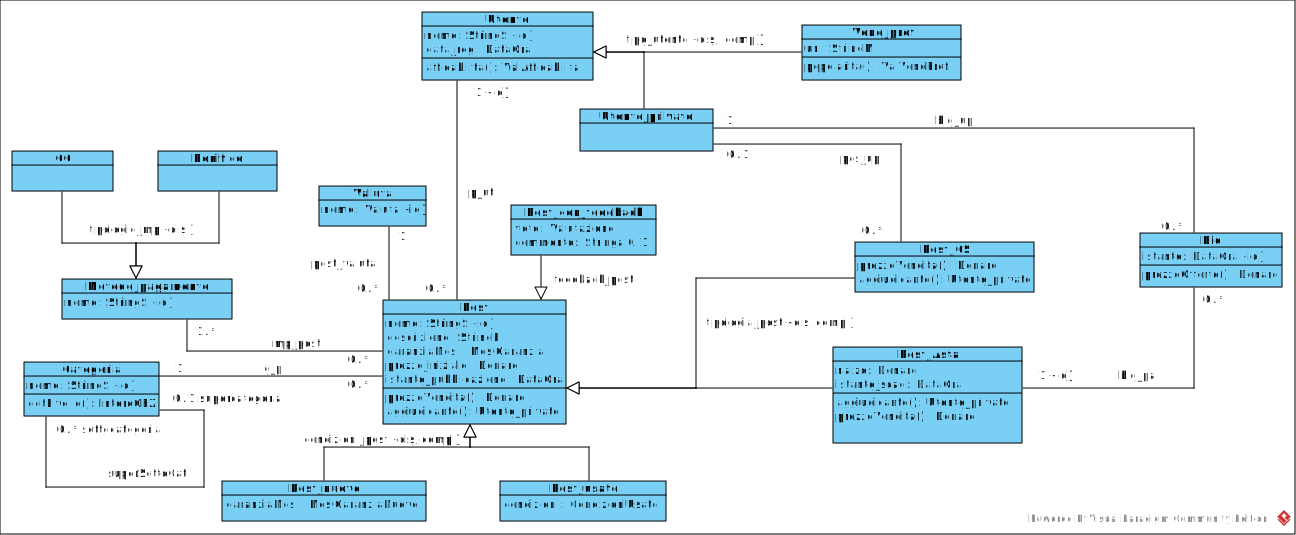
\includegraphics[width=\textwidth]{../Diagramma delle classi.pdf}
    \caption{Diagramma delle classi}
\end{figure}

\newpage
\section{Specifiche dei tipi di dati}

\begin{enumerate}
    \item ValutazioneNave Intero in [3,5]\label{sec:ValutazioneNave}
    \item InteroGEZ Intero in [0, +$\infty$]\label{sec:InteroGEZ}
    \item InteroGZ Intero in (0, +$\infty$)\label{sec:InteroGZ}
    \item Giorno \{Lun, Mar, Mer, Gio, Ven, Sab, Dom\}\label{sec:Giorno}
    \item Ora \{ora: intero in [0,23], minuti: intero in [0,59]\}\label{sec:Ora}
    \item StringaS varchar di lunghezza 100\label{sec:StringaS}
    \item StringaM varchar di lunghezza 500\label{sec:StringaM}
    \item StringaL varchar di lunghezza 1000\label{sec:StringaL}
    \item TipoCrocieraLunaDiMiele \{tradizionale, alternativa\}\label{sec:TipoCrocieraLunaDiMiele}
\end{enumerate}

\newpage
\section{Specifiche delle classi e delle associazioni}
\subsection*{Classe Crociera, \hyperref[sec:RequisitiCrociera]{v.req.1}}\label{sec:Crociera}
Tabella delle specifiche degli attributi:
\begin{table}[h]
    \centering
    \begin{tabular}{|c|c|c|c|}
        \hline
        Attributo & Tipo & Cardinalità & Descrizione \\
        \hline
        codice & StringaS & 1 & Codice della crociera \\
        data\_inizio & Data & 1 & Data di inizio della crociera \\
        data\_fine & Data & 1 & Data di fine della crociera \\
        \hline
    \end{tabular}
    \caption{Attributi della classe Crociera}
\end{table}

Tabella delle specifiche delle associazioni:
\begin{table}[h]
    \centering
    \begin{tabular}{|c|c|c|c|}
        \hline
        Associazione & Cardinalità & Descrizione \\
        \hline
        nave & 1 & La nave utilizzata per la crociera \\
        itinerario & 1 & L'itinerario della crociera \\
        prenotazioni & 0..* & Le prenotazioni della crociera \\
        \hline
    \end{tabular}
    \caption{Associazioni della classe Crociera}
\end{table}
\subsection*{Classe Nave, \hyperref[sec:RequisitiNave]{v.req.2}}\label{sec:Nave}
\subsection*{Classe Destinazione, \hyperref[sec:RequisitiDestinazione]{v.req.3}}\label{sec:Destinazione}
\subsection*{Classe Itinerario, \hyperref[sec:RequisitiItinerario]{v.req.4}}\label{sec:Itinerario}
\subsection*{Classe PostoDaVedere, \hyperref[sec:RequisitiPostoDaVedere]{v.req.5}}\label{sec:PostoDaVedere}
\subsection*{Classe Utente, \hyperref[sec:RequisitiUtente]{v.req.6}}\label{sec:Utente}
\subsection*{Classe Prenotazione, \hyperref[sec:RequisitiPrenotazione]{v.req.7}}\label{sec:Prenotazione}
\subsection*{Classe Città, \hyperref[sec:RequisitiCittà]{v.req.8}}\label{sec:Città}
\subsection*{Classe Nazione, \hyperref[sec:RequisitiNazione]{v.req.9}}\label{sec:Nazione}
\subsection*{Classe Continente, \hyperref[sec:RequisitiContinente]{v.req.10}}\label{sec:Continente}
\subsection*{Classe Porto, \hyperref[sec:RequisitiPorto]{v.req.11}}\label{sec:Porto}
\subsection*{Classe OrarioPostoDaVedere, \hyperref[sec:RequisitiOrarioPostoDaVedere]{v.req.12}}\label{sec:OrarioPostoDaVedere}
\subsection*{Classe Tappa, \hyperref[sec:RequisitiTappa]{v.req.13}}\label{sec:Tappa}

\newpage
\section{Specifiche dei vincoli esterni}

\begin{enumerate}
    \item V.Crociera.
    \begin{enumerate}
        \item V.Crociera.data\_inizio\_leq\_data\_fine.
        \begin{enumerate}
            \item data di inizio $\leq$ data di fine
        \end{enumerate}
        \item V.Crociera.prenotazioni\_leq\_numero\_massimo\_passeggeri.
        \begin{enumerate}
            \item La somma dei posti prenotati per la crociera $\leq$ numero massimo di passeggeri
        \end{enumerate}
    \end{enumerate}
    \item V.Nave.
    \item V.Destinazione.
    \item V.Itinerario.
    \item V.PostoDaVedere.
    \item V.Utente.
    \item V.Prenotazione.
    \begin{enumerate}
        \item V.Prenotazione.istante\_di\_prenotazione\_less\_data\_inizio\_crociera.
        \begin{enumerate}
            \item istante di prenotazione $<$ data di inizio crociera
        \end{enumerate}
    \end{enumerate}
    \item V.Città.
    \item V.Nazione.
    \item V.Continente.
    \item V.Porto.
    \item V.OrarioPostoDaVedere.
    \begin{enumerate}
        \item V.OrarioPostoDaVedere.ora\_inizio\_less\_ora\_fine.
        \begin{enumerate}
            \item ora di inizio $<$ ora di fine
        \end{enumerate}
    \end{enumerate}
    \item V.Tappa.
    \begin{enumerate}
        \item giorno di arrivo $\leq$ giorno di partenza
    \end{enumerate}
\end{enumerate}


\newpage
\section{Specifiche delle operazioni}

In questa sezione verranno descritte le operazioni che il sistema deve essere in grado di eseguire.
\newline
\newline
tipCrocLdM(): TipoCrocieraLunaDiMiele
\begin{enumerate}
    \item Pre: nessuna
    \item Post: no side effect
    \item Return:
    \begin{enumerate}
        \item se il numero di destinazioni romantiche $\geq$ il numero di destinazioni divertenti, restituisce tradizionale
        \item altrimenti, restituisce alternativa
    \end{enumerate}
\end{enumerate}

ordineTappa(): InteroGZ
\begin{enumerate}
    \item Pre: nessuna
    \item Post: no side effect
    \item Return:
    \begin{enumerate}
        \item sia I l'itinerario tale che tappa\_itin(this, I) = True
        \item sia T l'insieme delle tappe di I
        \item sia T' = \{t' $\in$ T: (giorno\_arrivo(t') $\leq$ giorno\_arrivo(t)) \newline $\lor$ (giorno\_arrivo(t') = giorno\_arrivo(t) $\land$ ora\_partenza(t') $\leq$ ora\_arrivo(t))\}
        \item restituisce la cardinalità di T'+1
    \end{enumerate}
\end{enumerate}



\end{document}